\chapter{Конструкторская часть}

\section{Требования к программному обеспечению}\label{section:requirements}

Программное обеспечение должно удовлетворять следующим функциональным требованиям: на входе -- матрица смежности и дополнительные параметры, необходимые для муравьиного алгоритма, на выходе -- длина кратчайшего маршрута и сам маршрут.

Программное обеспечение также должно соответствовать следующим требованиям:
\begin{itemize}[label=---]
	\item наличие пользовательского интерфейса для выбора действий;
	\item вывод длины минимального маршрута и самого маршрута;
	\item предоставление функционала для измерения времени выполнения алгоритмов.
\end{itemize}

\section{Разработка алгоритмов}
В данном разделе представлены схемы алгоритмов для полного перебора (рисунки \ref{img:bruteforce}, \ref{img:calculatepath}) и муравьиного алгоритма (рисунки \ref{img:ant1} -- \ref{img:ant4})

\begin{figure}[h]
	\centering
	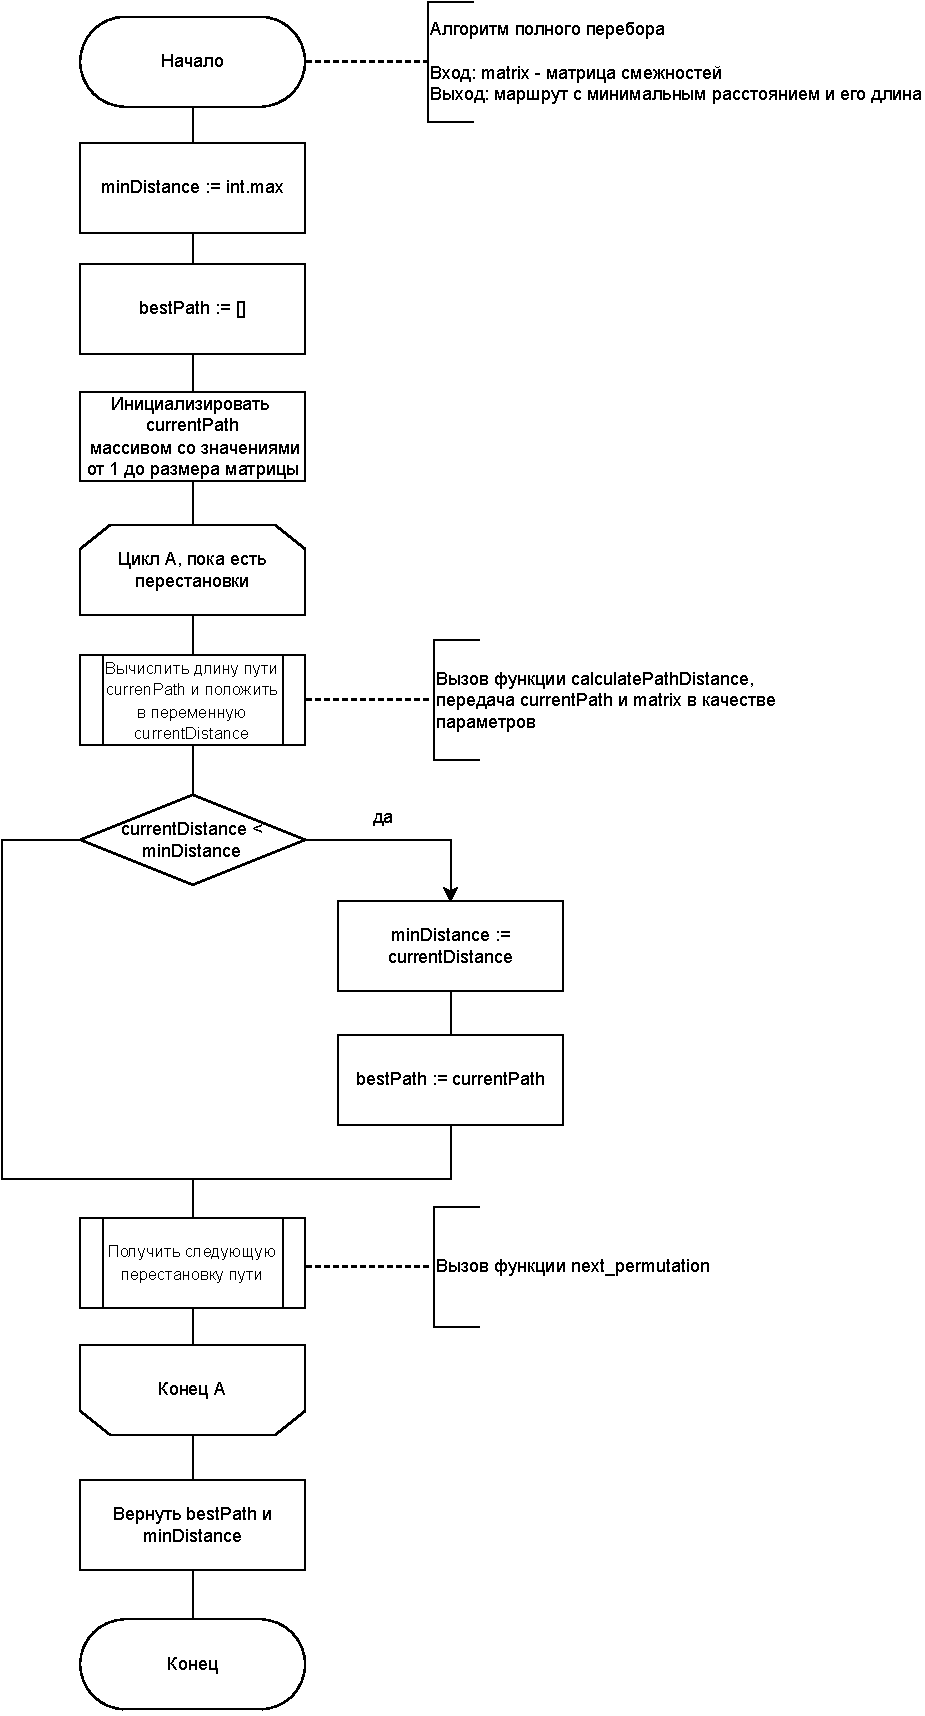
\includegraphics[width=0.8\linewidth]{img/bruteforce.pdf}
	\caption{Схема метода полным перебора}
	\label{img:bruteforce}
\end{figure}

\begin{figure}[h]
	\centering
	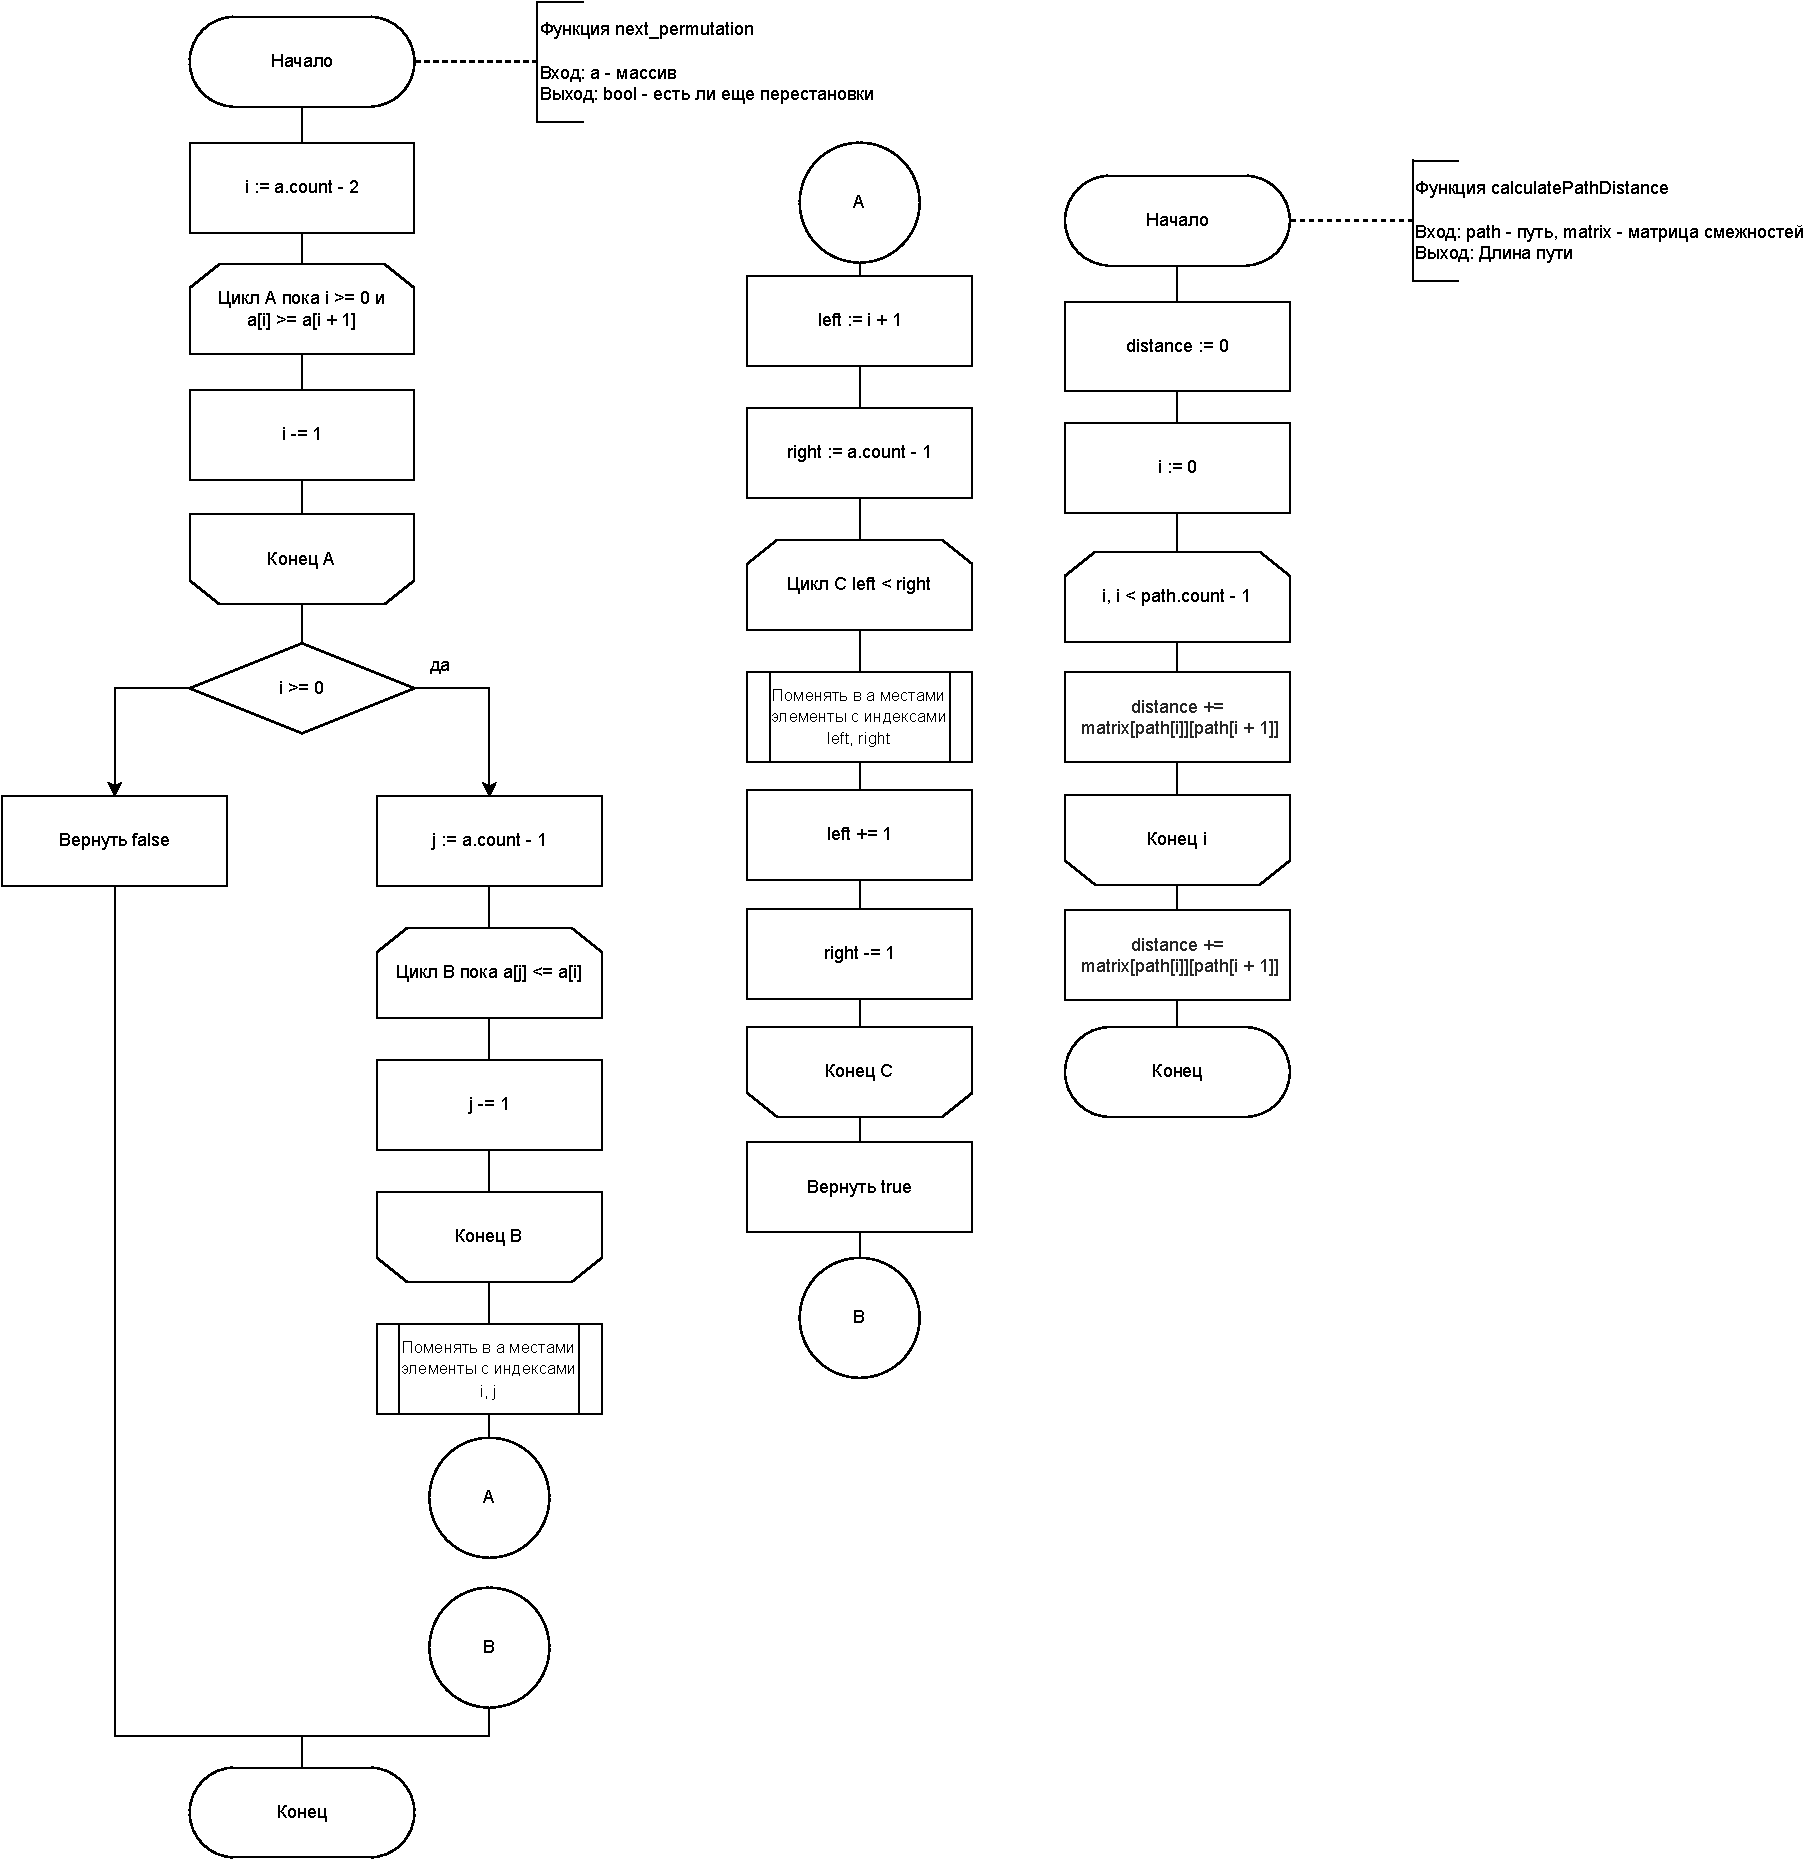
\includegraphics[width=1\linewidth]{img/calculatepath.pdf}
	\caption{Вспомогательные функции для метода полным перебором}
	\label{img:calculatepath}
\end{figure}

\begin{figure}[h]
	\centering
	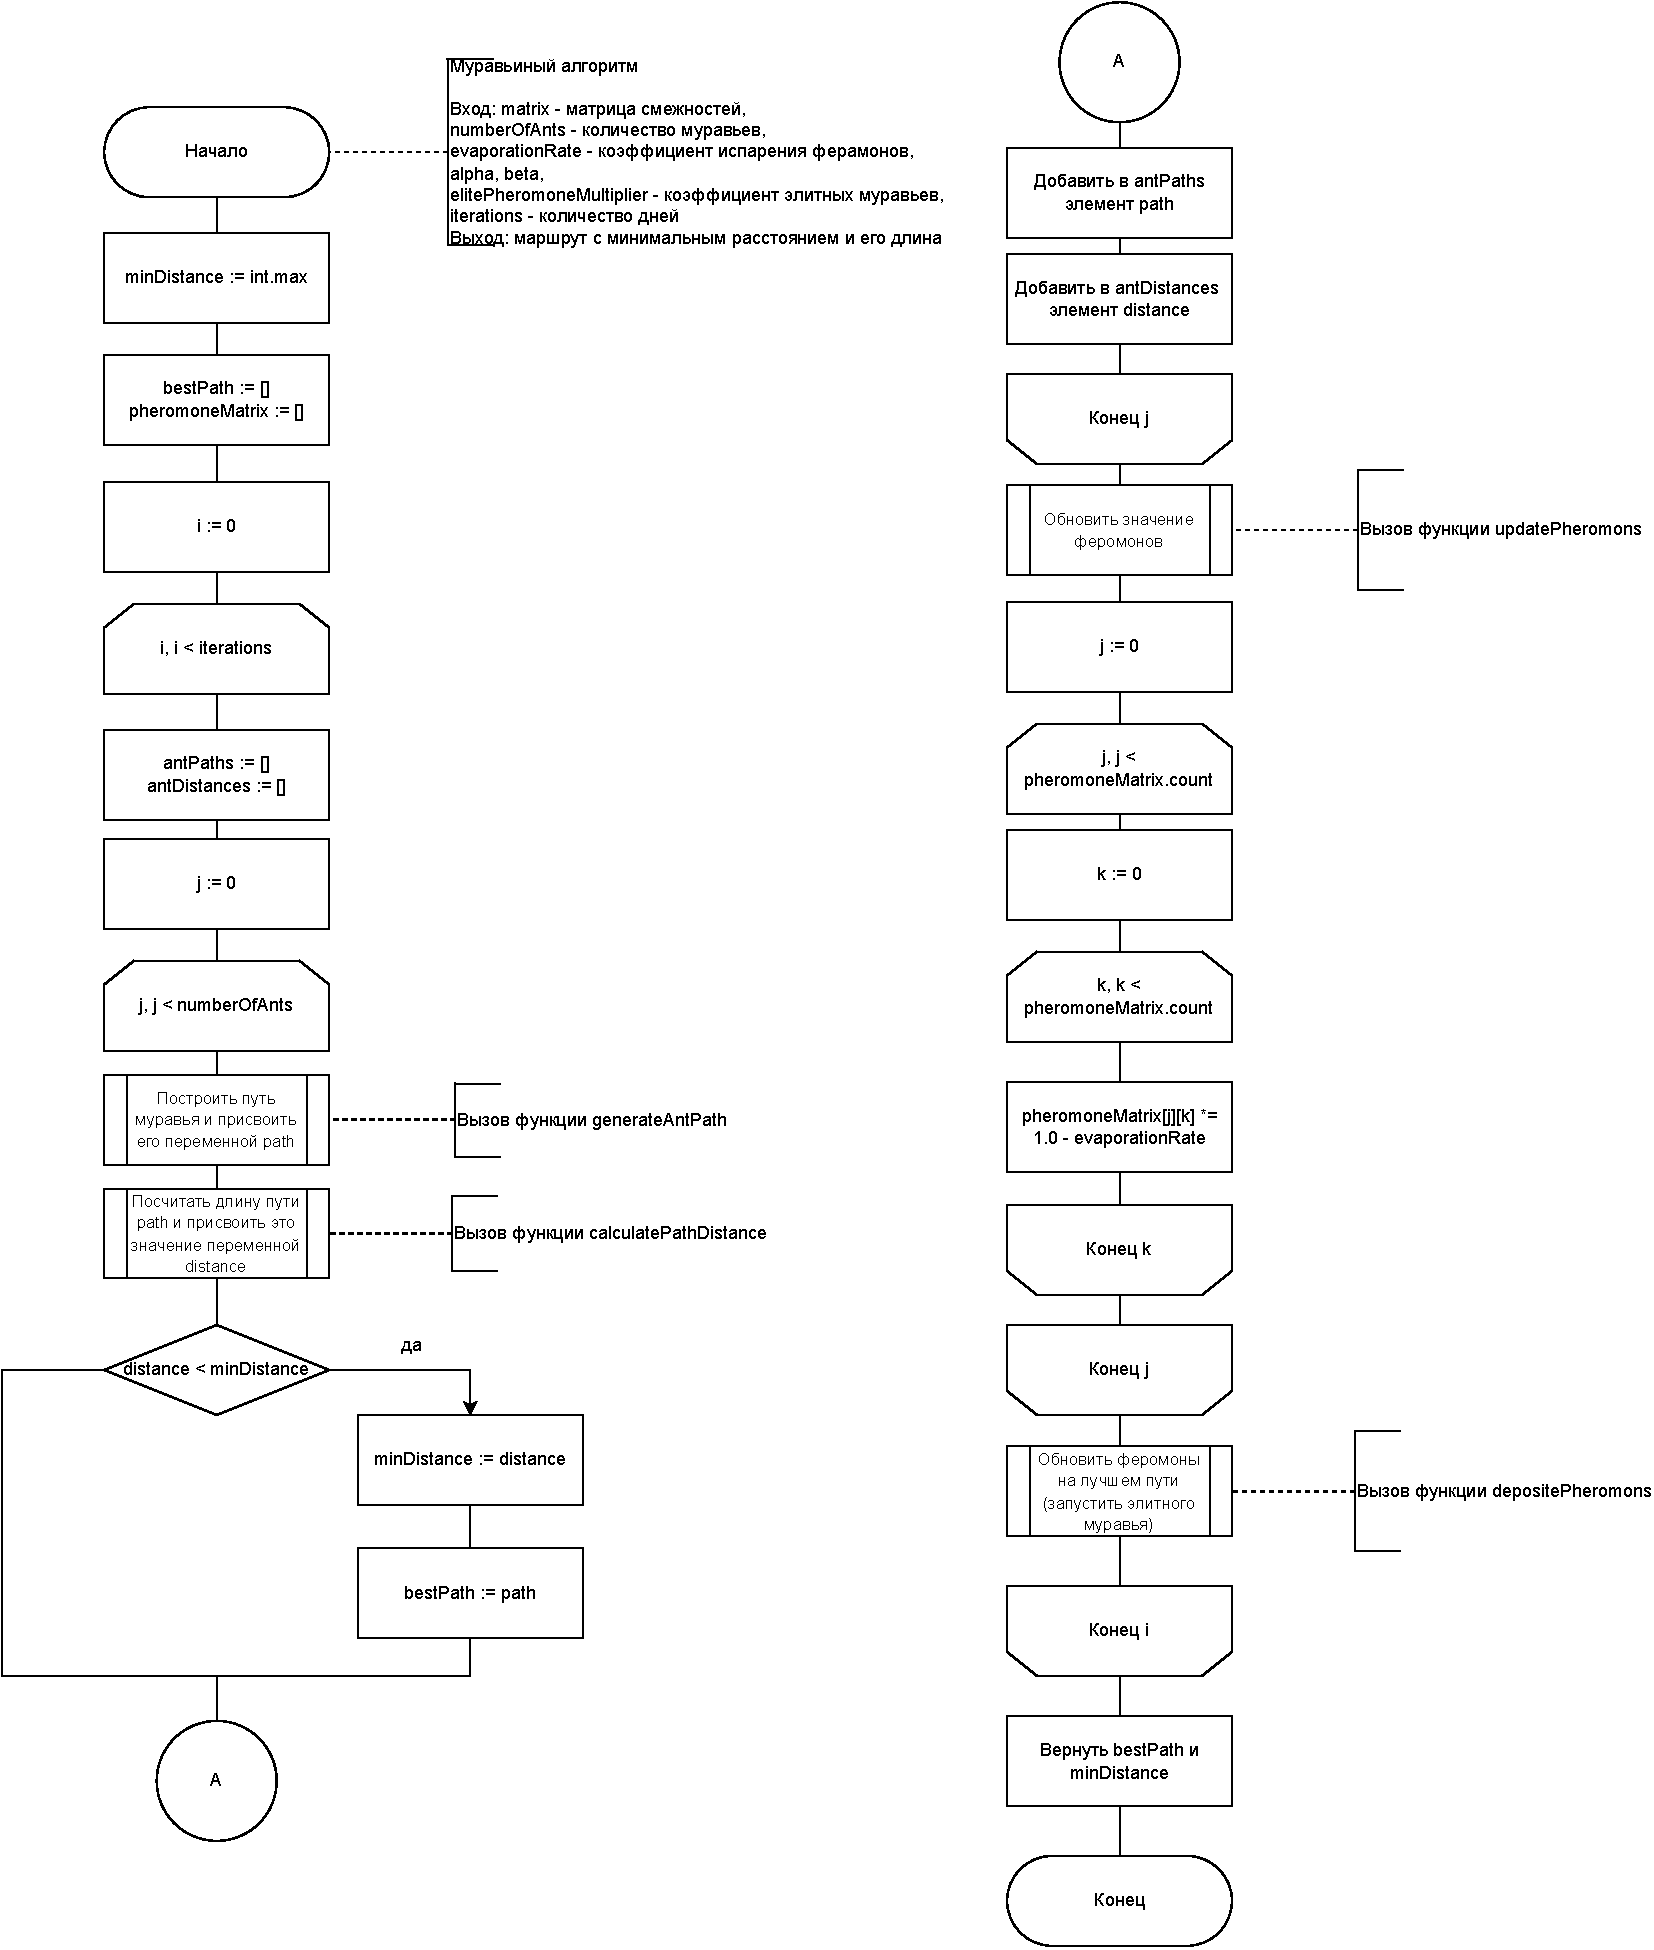
\includegraphics[width=1\linewidth]{img/ant1.pdf}
	\caption{Схема метода на основе муравьиного алгоритма}
	\label{img:ant1}
\end{figure}

\begin{figure}[h]
	\centering
	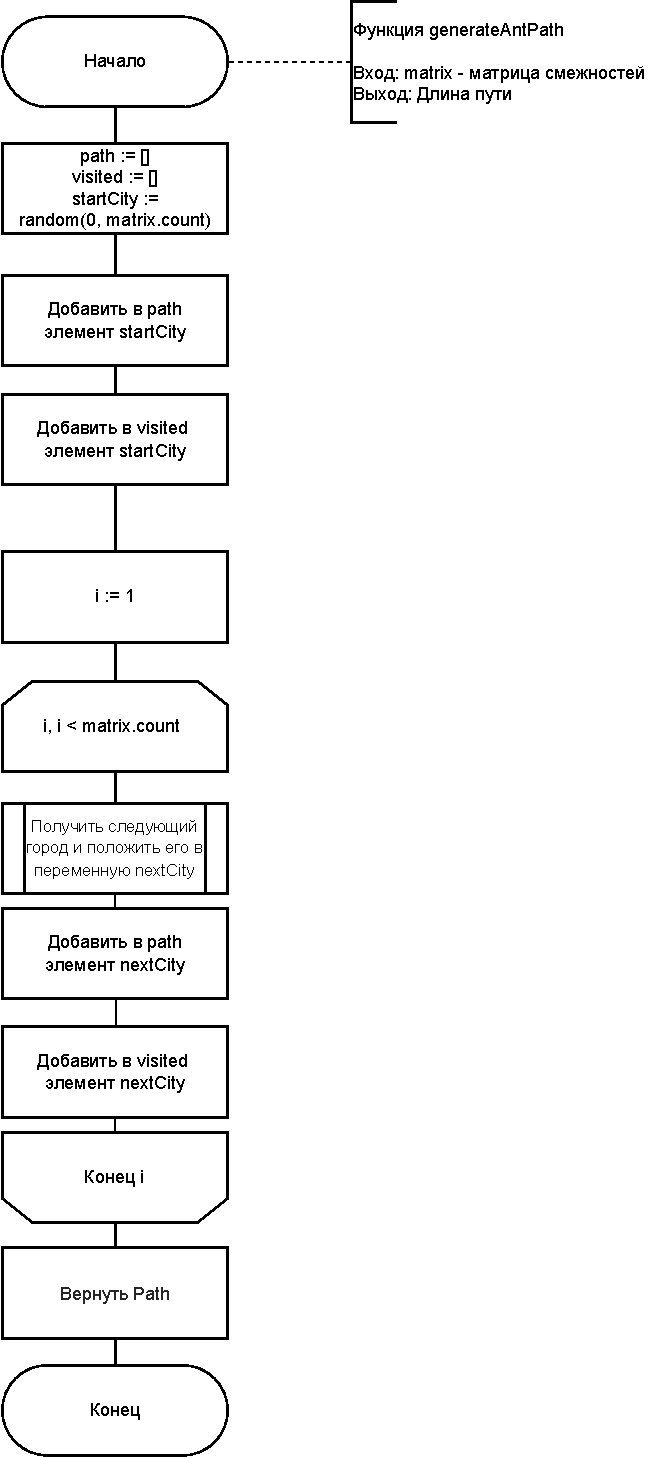
\includegraphics[width=0.6\linewidth]{img/ant2.pdf}
	\caption{Схема функции составления маршрута муравья}
	\label{img:ant2}
\end{figure}

\begin{figure}[h]
	\centering
	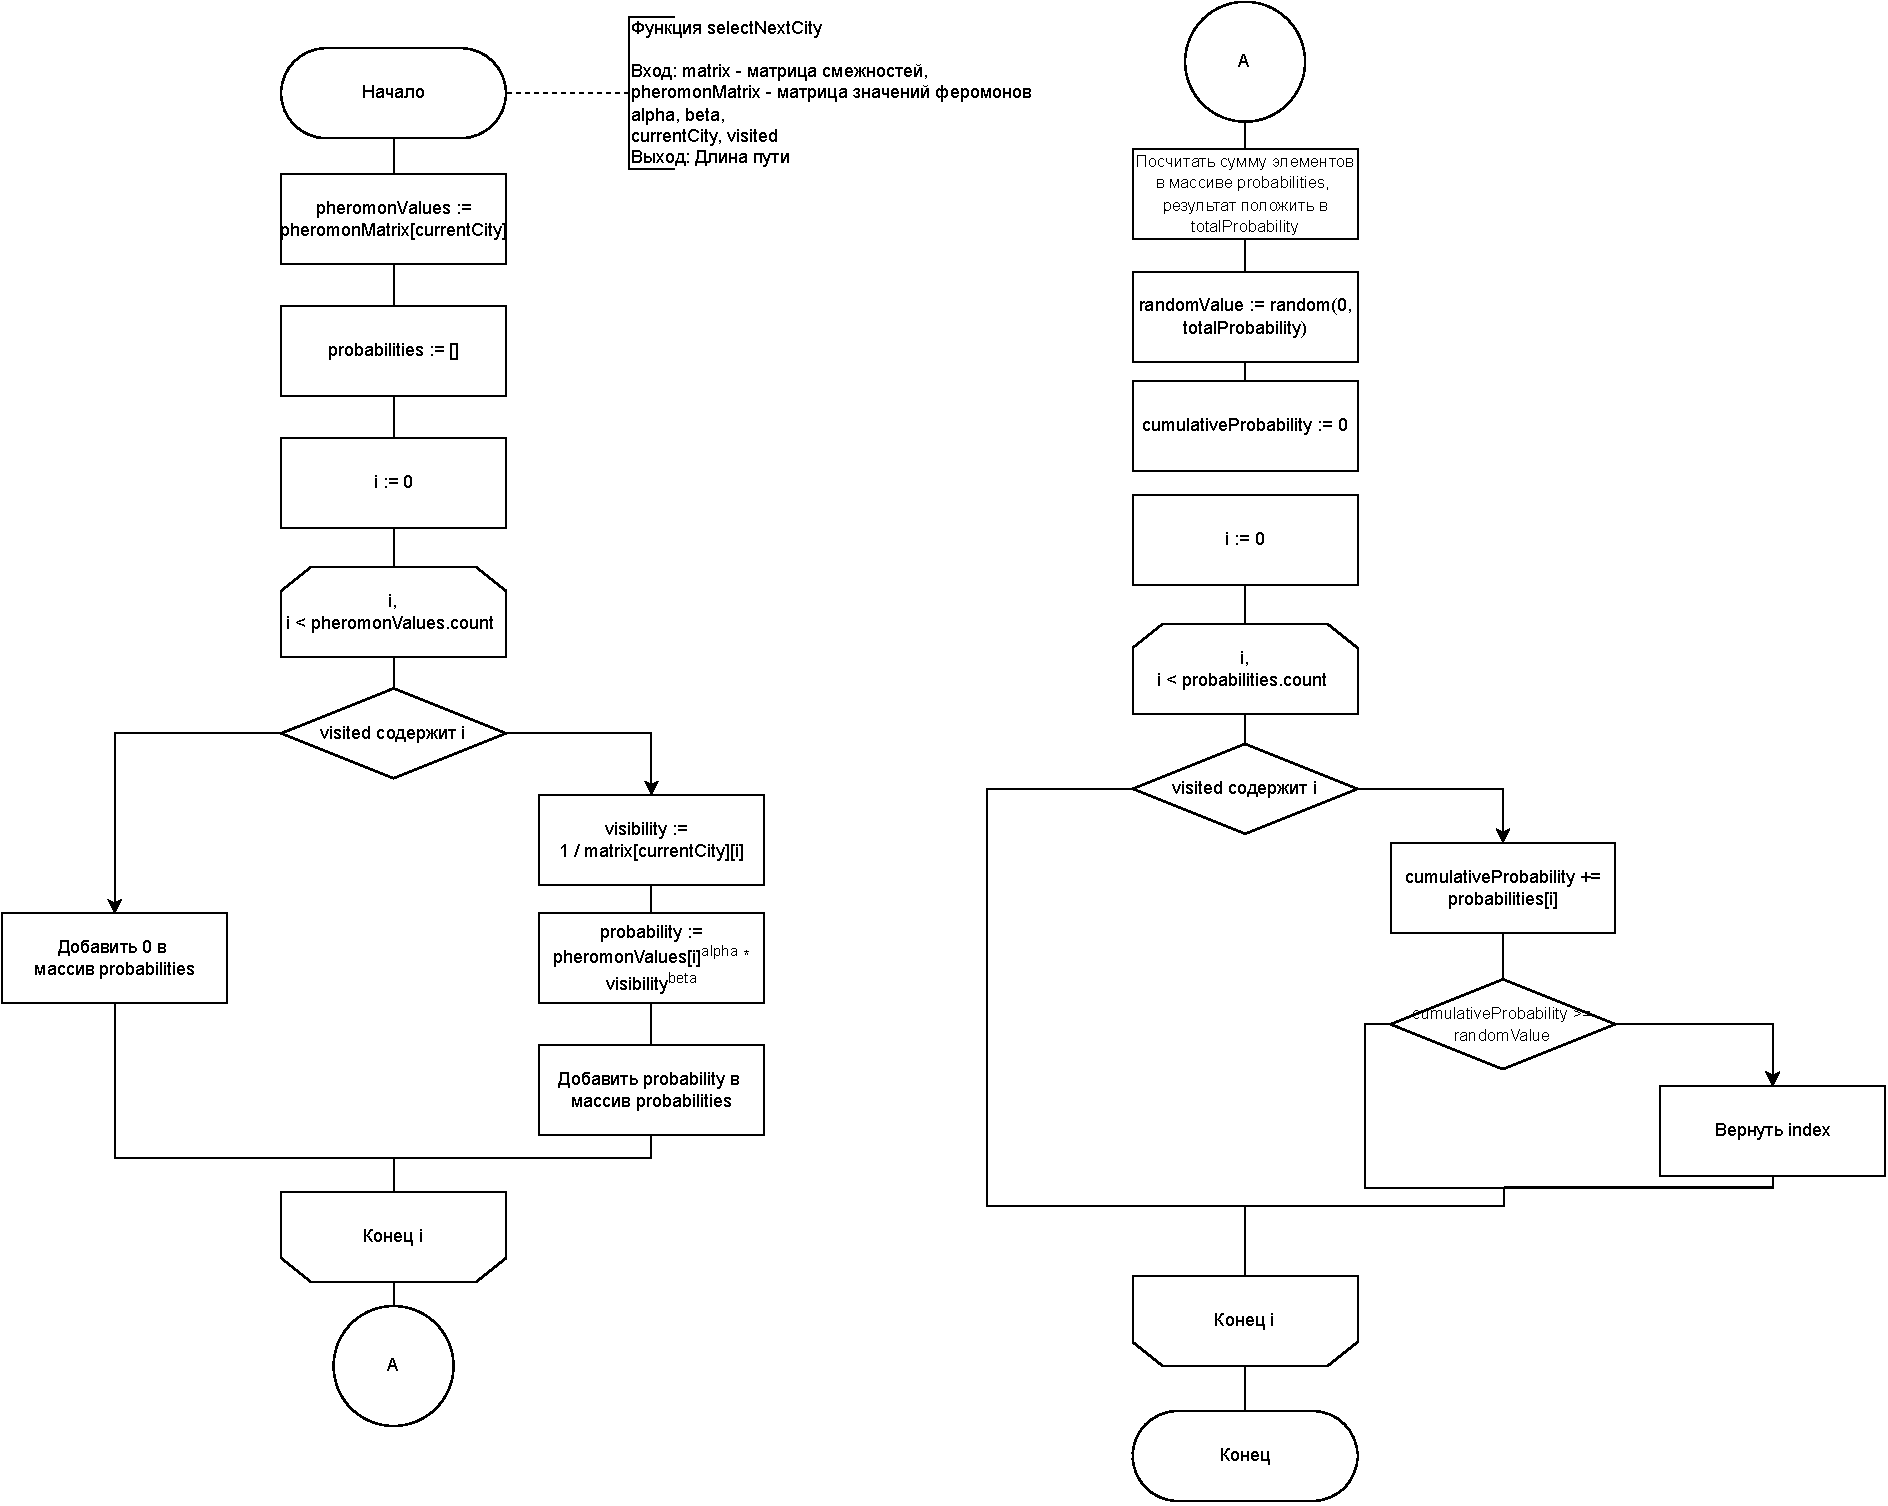
\includegraphics[width=1\linewidth]{img/ant3.pdf}
	\caption{Схема функции выбора следующего города}
	\label{img:ant3}
\end{figure}

\begin{figure}[h]
	\centering
	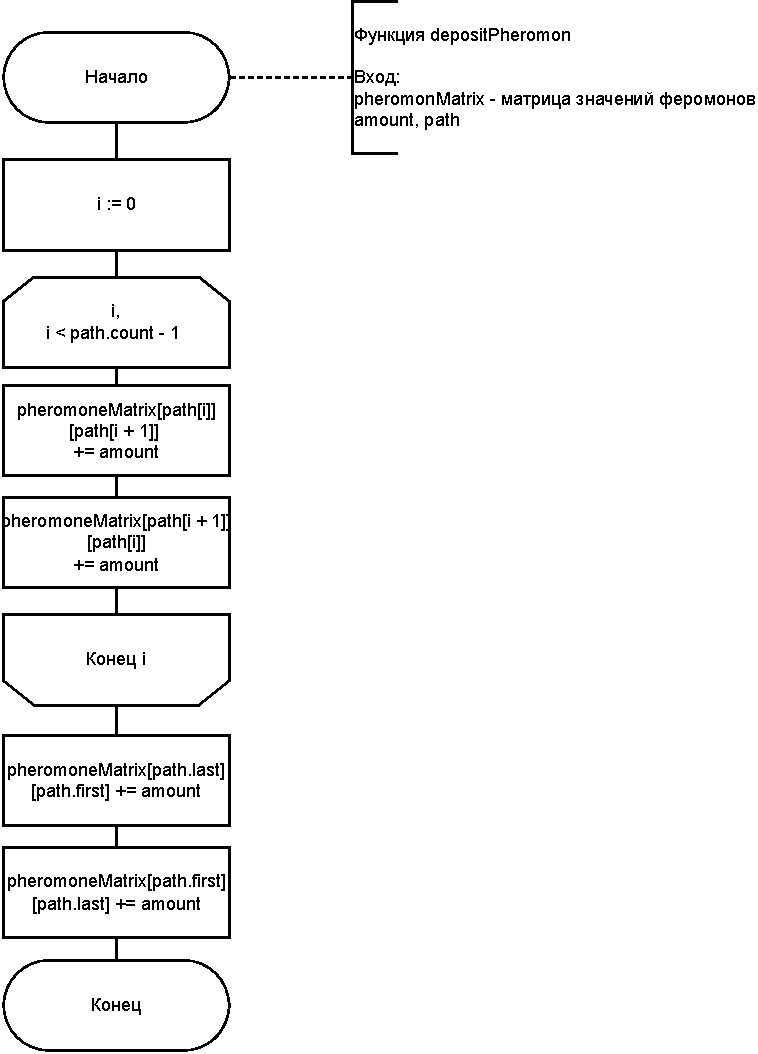
\includegraphics[width=1\linewidth]{img/ant4.pdf}
	\caption{Схема функции элитных муравьев}
	\label{img:ant4}
\end{figure}

\clearpage
\section*{Вывод}
В данном разделе были представлены схемы методов решения задачи коммивояжёра: полным перебором и на основе муравьиного алгоритма. 
